\documentclass[a4paper,10pt]{article}

\usepackage[T1]{fontenc}


%\renewcommand{\rmdefault}{ppl} %Palatino
%\renewcommand{\rmdefault}{cmfib} % computer modern fibonacci 365
%\renewcommand{\rmdefault}{\sfdefault} default serifenlos
\usepackage{ae}
\renewcommand{\familydefault}{phv} % Helvetica angenehm zu lesen ! 386
\usepackage{graphicx}

% Silbentrennung
\usepackage[english,ngerman]{babel}

% PDF
%LaTeX erzeugt mit dem hyperref-Paket interaktive PDF-Dateien mit Bookmarks
\usepackage{color}
\usepackage[colorlinks]{hyperref}
\usepackage{my} % modifizierte Ueberschriften
%\usepackage{avant}
%\usepackage{mathptmx}

%empfohlen aber gehen leider nicht:
%\usepackage{microtype} Optischer Randausgleich besserer Rand
%\usepackage{mparhack}


%Einstellungen der Seitenränder
% \usepackage[left=3cm,right=3cm,top=3cm,bottom=3cm,includeheadfoot]{geometry}

%Umlaute ermöglichen
\usepackage[latin1]{inputenc}
\usepackage{tabularx} % Seite 259 im Latex Buch, ist extrem cool !!
\newcolumntype{Y}{>{\small\raggedright\arraybackslash}X}


%Kopf- und Fußzeile
\usepackage{fancyhdr}
\pagestyle{fancy}
\fancyhf{}

%Kopfzeile mittig
\fancyhead[C]{\nouppercase{\leftmark}}
%Linie oben
\renewcommand{\headrulewidth}{0.5pt}

%Fußzeile mittig
\fancyfoot[C]{\thepage}
%Linie unten
\renewcommand{\footrulewidth}{0.5pt}





\begin{document}

{\sc Die Schriftart small caps (Kapit"alchen).}
{\sf Die Schriftart sans serif (serifenlos).}

\tableofcontents
\newpage

TODO:

Welchen typen unterstuetzen wir
Alle Ausdruecke werden bei uns in der Klasse Symboltable ueberprueft auf Korrektheit. 


\section{Parser}

The first set is very interesting for a top down parser. The parser compares the actual token with the first-sets symbol and takes decisions between alternatives. To guarantee that the decision between two alternatives is correct, the first set of the alternatives must be disjunctive. 

% TODO umschreiben (ANFANG)
%We defined the first-sets and follow-sets to check that we can really achieve that a lookahead of one symbol is sufficient.

%The first set very interesting for a top down analysis, because it determines the progress of the analysis.
%The first set of a node contains all token, by which the parser will be guided to the node.

%If the actual text isn't matched by one of the token of the first set, an other node will be chosen, namely the node with the first set that contains a token, which matches. If there is no such alternative the parsing is stopped with an error message. To guarantee that the decision between alternatives is definite, the first sets of the alternatives must be disjunctive, i.e.: there may not be a token contained in two alternative first sets. 

% TODO umschreiben (ENDE)

\subsection{First Sets}

% use packages: array
\begin{tabular}{p{4cm}l}
	S & First(S) \\ \hline
	& \\
	program & package\_declaration package\_import  \\
	package\_declaration & "package" \\
	package\_import & "import" \\
	class\_declaration & "public" \\
	class\_block & method\_declaration datatype\_declaration \\
	method\_declaration & "public" \\
	datatype\_declaration & "static" datatype\_decsriptor \\
	method\_call & identifier \\
	datatype\_assignment & identifier \\
	body\_block & while\_statement if\_statement return\_statement datatype\_declaration identifier (method\_call datatype\_assignment) \\
	while\_statement & "while" \\
	if\_statement & "if" \\
	return\_statement & "return" \\
	datatype\_decsriptor & datatype \\
	datatype & primitive object \\
	primitive & "int" "boolean" "char" \\
	object & String identifier \\
	identifier & letter \\
	selector & "." "[" \\
	condition & expression \\
	expression & term \\
	term & factor \\
	factor & value \\
	value & identifier datatype not\_value TODO \\
	integer & "-" digit\_non\_zero \\
	char & "'"\\
	boolean & "true" "false" \\
	string & """ \\
	digit & digit\_non\_zero digit\_zero \\
	digit\_non\_zero & 1 2 3 4 5 6 7 8 9 \\
	digit\_zero & 0 \\
\end{tabular}


\begin{figure}
	\begin{center}
	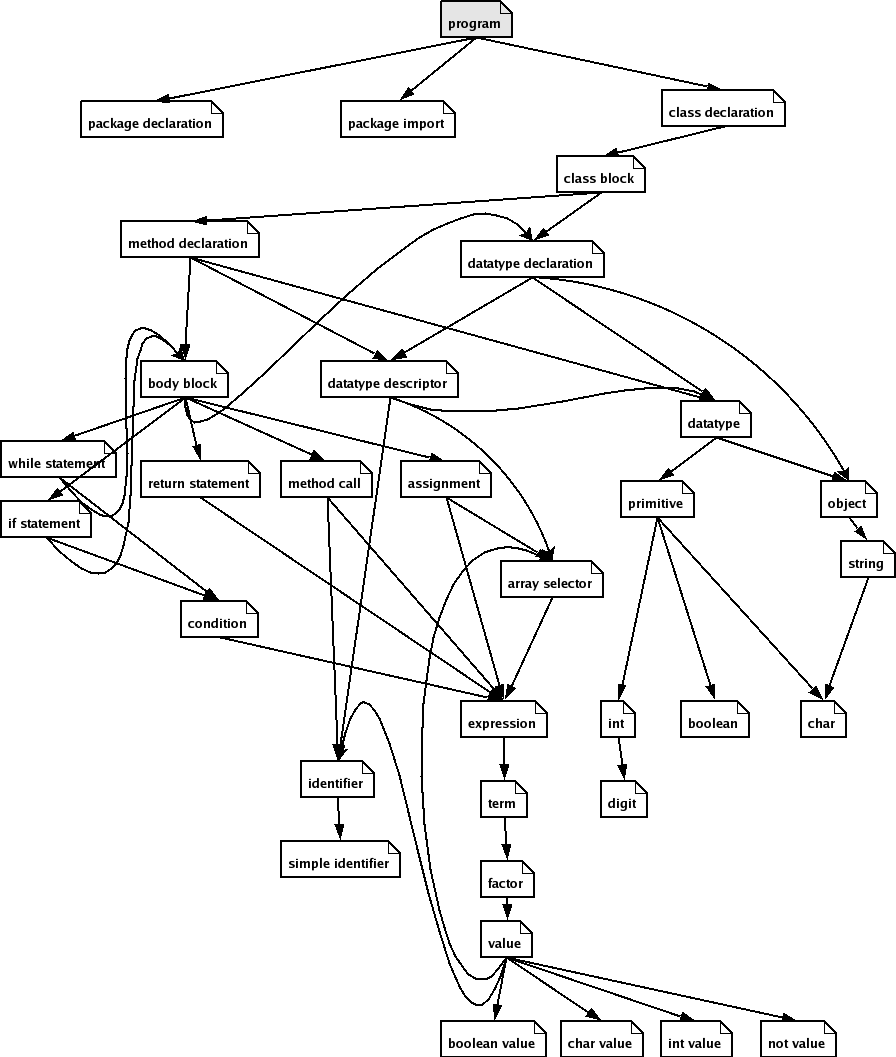
\includegraphics[scale=0.4]{Diagram_Small.png}
% Diagram_Small.eps: 300dpi, width=10.83cm, height=12.67cm, bb=0 0 1279 1497 ,bb=0 0 1279 1497
% width=15cm,height=15cm
	
	\label{dep_diagram}
	\caption {Dependencies representation of parsing procedures (simplified).}
	\end{center}
\end{figure}

\section{Memorymanagement in comPiler}
ComPiler compiles code for RISC-based architectures. It has 32 registers each
with size 32 Bit (4 Byte). Register 0 (R0) has always the value 0. Register 31
(R31) is reserved for return addresses. In a branch instruction the PC is stored
in R31. 

The instruction register (IR) holds the current instruction being executed. \newline 
The program counter (PC) contains the address of the instruction to be
fetched next. \newline
The stack pointer (SP) indicates the top element of a register-based stack. That
means that on some occasions registers are accessed like a stack and the SP
points out the next free register.  
\newline
The memory for the activation frames is organized like a stack. Each frame is an
entry. The SP indicates the next free memory and the FP the base address of the
current frame. 
\subsubsection{Organization of an activation frame}
An activation frame is a special memory context used for a procedure and its
local variables. It's created by a branch instruction (e.g. a procedure call). The base address of the activation 
frame is also the base address for all local variables declared here. Because this base address is highly 
important and one needs to access it efficently it's saved in the frame pointer (FP).
As the former PC was saved at the branch instruction, we use it as our return
address and save it in R31.



\subsection{local variables}
ComPiler offers local hiding of variables. That means, that procedures can
contain variables that cannot be seen outside the procedure. Even if there
exists a variable with the same name outside the procedure, these two don't
interfere. 
\subsubsection*{So what happens when a branch instruction occurs?}
When the instruction is executed, the PC is stored in R31. Then the code
generator jumps to the next instruction-address indicated by the branch instruction.
Now we have entered a special memory context for procedures (an activation frame). In this frame all memory is 
managed that is needed in the procedure
\newline
  
 


Local variables have the following properties: 
\begin{itemize}
  \item They have negative offsets to their baseaddresses
\end{itemize}



\section{The symbolfile}
The symbolfile (file-extension is .sym)is a sequential representation of the
symboltable. All entries
are representations of the symbols found in the sourcecode. \\
Because the symbolfile is just read one time during compilation, it cannot be
seen as a performance factor. So we decided to write the symbolfile in
xml-format as it is a good representation of objects. 
\subsection{Structure}
The root-tag of the symbolfile is \emph{<symbolfile>}. After the xml-header and
the root-tag the symbolfile starts with a list of the so-called \emph{module anchors}. Every
module anchor represents a module that's imported. In xml-syntax this lookes
like that:
\begin{lstlisting}[caption={module anchors}]
<modules>
	<module>
		<name> modulename 1 </name>
	</module>
	<module>
		<name> modulename 2 </name>
	</module>
	<module>
		<name> modulename 3 </name>
	</module>
</modules>
\end{lstlisting}

After the module anchors the actual symboltable representation starts. It is
enclosed in a \emph{<symbols>}-tag There are 3 different elementtypes that can be described here:
\begin{itemize}
  \item variables
  \item arrays
  \item methods 
\end{itemize}
\subsubsection{variables}
A variable has 2 properties: 
\begin{itemize}
  \item one of the primitive datatypes like \emph{boolean}, \emph{int} or \emph{char}
  \item the name of the variable in the sourcecode
\end{itemize}

\begin{lstlisting}[caption={variables}]
<variable>
	<type> type </type>
	<name> name </name>
</variable>
\end{lstlisting}

\subsubsection{arrays}
An array has 3 properties
\begin{itemize}
  \item one of the primitive datatypes like \emph{boolean}, \emph{int} or \emph{char}
  \item the name of the variable in the sourcecode
  \item the number of elements in the array
\end{itemize}

\begin{lstlisting}[caption={arrays}]
<array>
	<type> type </type>
	<name> name </name>
	<size> size </size>
</array>
\end{lstlisting}

\subsubsection{methods}
An array has 3 properties and contains another symboltable with the parameters
of the method. 
\begin{itemize}
  \item the return value of the method as one of the primitive datatypes
  like \emph{boolean}, \emph{int} or \emph{char}
  \item the name of the method in the sourcecode
  \item the number of elements in the array
\end{itemize}
So the description of a method is a recursive search through the symboltable.

\begin{lstlisting}[caption={methods}]
<method>
	<type> type </type>
	<name> name </name>
	<size> size </size>
	<symbols>
		<variable>
			<type> type </type>
			<name> name </name>
		<variable>
	</symbols>
</method>
\end{lstlisting}



\end{document}
